% ============================================================
% STATISTICAL METHODS REVIEW — Summary Table and Figure
% Insert into Chapter 3 or use as reference appendix material
% ============================================================

% ============================================================
% OPTION A: SUMMARY TABLE
% ============================================================
\begin{table}[htbp]
\centering
\caption{Summary of Statistical Methods, Appropriateness, and Identified Issues}
\label{tab:stat_methods_review}
\footnotesize
\setlength{\tabcolsep}{3pt}
\renewcommand{\arraystretch}{1.25}
\resizebox{\textwidth}{!}{%
\begin{tabular}{p{2.0cm} p{2.2cm} p{2.2cm} p{1.5cm} p{1.5cm} p{2.0cm} p{3.0cm} p{3.0cm}}
\toprule
\textbf{Test / Metric} &
\textbf{Purpose} &
\textbf{Design} &
\textbf{Effect Size} &
\textbf{$n$} &
\textbf{Key Assumptions} &
\textbf{Verdict} &
\textbf{Issues / Recommendations} \\
\midrule

% --- MCQ Robustness ---
\multicolumn{8}{l}{\textit{\textbf{MCQ Robustness (Objective 5a)}}} \\
\addlinespace[0.3em]

Chi-square test of independence &
Global: aggregate correctness $\times$ position &
$k \times 2$ contingency table; $k$ = number of variants &
Cram\'{e}r's $V$ &
5{,}720 per model\textsuperscript{a} &
Expected cell counts $\geq 5$; independent observations &
\textbf{Appropriate with caveat}\textsuperscript{b} &
(1)~Methods say 4 variants but code uses 5 (includes baseline). (2)~Items appear across variants $\rightarrow$ observations not strictly independent; mitigated by Friedman complement. (3)~$\text{dof}=4$ confirms 5-level factor. \\
\addlinespace

Friedman test &
Within-item: repeated-measures correctness across rotated positions &
$N$ items $\times$ $k{=}4$ conditions; binary outcomes &
Kendall's $W$ &
$N{=}1{,}144$ items, $k{=}4$ &
Same items measured under all conditions; ordinal/binary outcomes &
\textbf{Appropriate} (equivalent to Cochran's $Q$ for binary data) &
(1)~Could be labeled Cochran's $Q$ for precision. (2)~Uses full 1{,}144 items (not 845 matched subset). (3)~$W$ computed correctly: $W = Q / [N(k{-}1)]$ verified numerically. \\
\addlinespace

% --- Effect size thresholds ---
$V$ and $W$ thresholds ($< 0.10$, $0.10$--$0.30$, $\geq 0.30$) &
Classify practical magnitude &
Predefined decision rubric &
--- &
--- &
Thresholds are domain-appropriate &
\textbf{Defensible} &
(1)~Aligned with Cohen's small/medium/large for $\phi$ / $w$. (2)~No CIs on $V$ or $W$ reported; recommend bootstrap CIs. \\
\addlinespace

% --- Multiple comparisons ---
Multiple testing (19 models $\times$ 2 tests) &
Family-wise error control &
38 total tests at $\alpha = 0.05$ &
--- &
--- &
Tests are independent across models &
\textbf{Needs attention} &
(1)~Expected $\sim$2 false positives under $H_0$. (2)~Borderline $p$-values (e.g., $p{=}0.032$) could flip under Holm correction. (3)~Recommend Holm--Bonferroni or BH/FDR, or justify per-model testing as separate confirmatory analyses. \\

\midrule

% --- Inter-Judge Reliability ---
\multicolumn{8}{l}{\textit{\textbf{Inter-Judge Reliability (Objective 4)}}} \\
\addlinespace[0.3em]

Spearman $\rho$ &
Rank-order agreement between 2 judges &
Pairwise correlation of total scores &
--- &
$n{=}16{,}051$\textsuperscript{c} &
Ordinal or continuous data; monotonic relationship &
\textbf{Appropriate but incomplete} &
(1)~$n{=}16{,}051$ makes $p$-value vacuous (any $\rho > 0$ is ``significant''). (2)~$\rho$ measures rank agreement, not absolute calibration. (3)~Recommend adding ICC(2,1) for absolute agreement and reporting CIs. \\
\addlinespace

Score distribution diagnostics &
Assess instrument discrimination &
Modality, spread, compression, skewness per model-judge &
--- &
--- &
--- &
\textbf{Described in Methods but missing from Results} &
(1)~Methods (Sec.~3.6) promise these diagnostics; Chapter~4 does not report them systematically. (2)~Add or remove from Methods. \\

\midrule

% --- Cross-Modality Comparison ---
\multicolumn{8}{l}{\textit{\textbf{Cross-Modality Comparison (Objective 5b)}}} \\
\addlinespace[0.3em]

Pearson $r$ &
Linear association: MCQ accuracy vs.\ normalized OSQ score &
Model-level aggregates &
--- &
$n{=}19$ &
Bivariate normality; interval data &
\textbf{Appropriate but low power} &
(1)~95\% CI for $r{=}0.80$ at $n{=}19$: $\approx (0.54, 0.92)$. (2)~No CIs reported. (3)~Power to detect $r{=}0.50$: $\approx$60\%. \\
\addlinespace

Spearman $\rho_s$ &
Rank agreement in model ordering &
Model-level ranks &
--- &
$n{=}19$ &
Monotonic relationship &
\textbf{Appropriate; same power concern} &
Consistent with Pearson analysis. \\
\addlinespace

Wilcoxon signed-rank &
Paired format difference: MCQ vs.\ OSQ per model &
$\Delta_i = \text{Acc}_{\text{MCQ},i} - \bar{S}'_{\text{OSQ},i}$ &
$d = \bar{\Delta}/s_{\Delta}$ (defined) &
$n{=}19$ &
Symmetric difference distribution; $\geq$10 non-zero pairs &
\textbf{Appropriate; notable finding} &
(1)~Test stat $= 0.0$ means \textit{all} 19 $\Delta_i > 0$ (MCQ always $>$ OSQ). (2)~Effect size $d$ is defined in Methods but \textbf{not reported in Ch.~4}. (3)~At $n{=}19$, minimum detectable $|d|$ at 80\% power $\approx 0.68$. \\
\addlinespace

$R^2$ (OLS) &
Variance explained: MCQ $\rightarrow$ OSQ &
Simple linear regression &
--- &
$n{=}19$ &
Linear relationship; normal residuals &
\textbf{Descriptive; acceptable} &
Reported as $R^2{=}0.671$ with $p$-value; no issues. \\
\addlinespace

Cross-modality classification rubric &
Categorize convergent / partially convergent / divergent &
Joint assessment of $r$, $\rho_s$, $|d|$, and Wilcoxon $p$ &
--- &
--- &
--- &
\textbf{Well-designed but not yet applied} &
Table~3.7 defines the rubric; Chapter~4 does not apply it to produce the final classification. \\

\midrule

% --- Token Efficiency ---
\multicolumn{8}{l}{\textit{\textbf{Token Efficiency (Objective 6)}}} \\
\addlinespace[0.3em]

Tokens-per-score &
Scalar efficiency metric &
$\overline{T}_{\text{total}} / \overline{S}_{\text{OSQ}}$ &
--- &
19 models &
Meaningful OSQ score denominator &
\textbf{Defined but not computed in Ch.~4} &
Recommend reporting or removing from Methods. \\
\addlinespace

Pareto frontier &
Identify non-dominated models in quality--token space &
Decision-analytic construct &
--- &
19 models &
--- &
\textbf{Appropriate} &
Not a statistical test; correctly used as a decision tool. \\

\bottomrule
\end{tabular}
}

\vspace{0.5em}
\footnotesize
\textit{Notes.}
\textsuperscript{a}~$n{=}5{,}720{=}5 \times 1{,}144$: code includes the original (baseline) dataset plus four rotated variants, yielding 5 conditions. Methods text describes only 4.
\textsuperscript{b}~The chi-square assumption of independent observations is technically violated because the same items appear across variants. The Friedman test (repeated-measures complement) addresses this, but the pairing should be acknowledged.
\textsuperscript{c}~$n{=}16{,}051 \approx 19 \times 845 - 4$: total item--model pairs scored by both judges, with 4 exclusions due to model/judge errors.
\end{table}


% ============================================================
% OPTION B: SUMMARY FIGURE (Statistical Analysis Pipeline — 2×2 Quadrant)
% ============================================================
\begin{figure}[htbp]
\centering
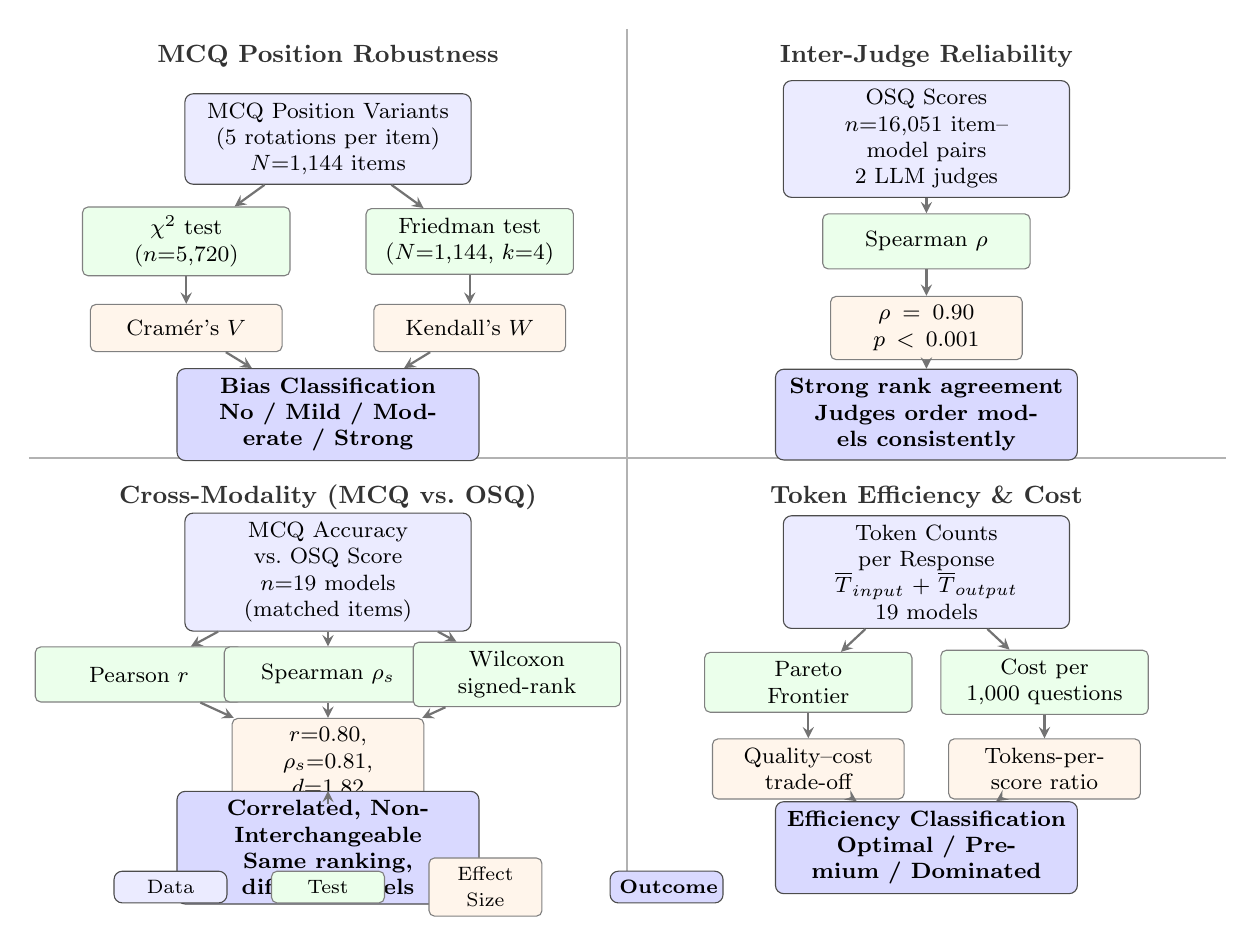
\begin{tikzpicture}[
    every node/.style={font=\footnotesize},
    data/.style={rectangle, draw=black!70, fill=blue!8, text width=3.4cm, minimum height=0.85cm, align=center, rounded corners=3pt},
    test/.style={rectangle, draw=black!50, fill=green!8, text width=2.4cm, minimum height=0.7cm, align=center, rounded corners=2pt},
    effect/.style={rectangle, draw=black!50, fill=orange!8, text width=2.2cm, minimum height=0.6cm, align=center, rounded corners=2pt},
    outcome/.style={rectangle, draw=black!70, fill=blue!15, text width=3.6cm, minimum height=0.85cm, align=center, rounded corners=3pt, font=\footnotesize\bfseries},
    quadlabel/.style={font=\small\bfseries, text=black!80},
    arrow/.style={->, >=stealth, thick, black!55},
]

% ── Quadrant frame ──
\draw[black!30, thick] (-7.6, 0.15) -- (7.6, 0.15);    % horizontal divider
\draw[black!30, thick] (0, 5.6) -- (0, -5.5);           % vertical divider

% ===================================================================
% TOP LEFT — MCQ Robustness
% ===================================================================
\node[quadlabel] at (-3.8, 5.25) {MCQ Position Robustness};

\node[data] (mcq_data) at (-3.8, 4.2) {MCQ Position Variants\\(5 rotations per item)\\$N{=}1{,}144$ items};

\node[test] (chi2) at (-5.6, 2.9) {$\chi^2$ test\\($n{=}5{,}720$)};
\node[test] (friedman) at (-2.0, 2.9) {Friedman test\\($N{=}1{,}144$, $k{=}4$)};

\node[effect] (cramv) at (-5.6, 1.8) {Cram\'{e}r's $V$};
\node[effect] (kendw) at (-2.0, 1.8) {Kendall's $W$};

\node[outcome] (classify1) at (-3.8, 0.7) {Bias Classification\\{\footnotesize No / Mild / Moderate / Strong}};

\draw[arrow] (mcq_data) -- (chi2);
\draw[arrow] (mcq_data) -- (friedman);
\draw[arrow] (chi2) -- (cramv);
\draw[arrow] (friedman) -- (kendw);
\draw[arrow] (cramv) -- (classify1);
\draw[arrow] (kendw) -- (classify1);

% ===================================================================
% TOP RIGHT — Inter-Judge Reliability
% ===================================================================
\node[quadlabel] at (3.8, 5.25) {Inter-Judge Reliability};

\node[data] (judge_data) at (3.8, 4.2) {OSQ Scores\\$n{=}16{,}051$ item--model pairs\\2 LLM judges};

\node[test] (spearman_j) at (3.8, 2.9) {Spearman $\rho$};

\node[effect] (rho_val) at (3.8, 1.8) {$\rho = 0.90$\\$p < 0.001$};

\node[outcome] (judge_out) at (3.8, 0.7) {Strong rank agreement\\{\footnotesize Judges order models consistently}};

\draw[arrow] (judge_data) -- (spearman_j);
\draw[arrow] (spearman_j) -- (rho_val);
\draw[arrow] (rho_val) -- (judge_out);

% ===================================================================
% BOTTOM LEFT — Cross-Modality Comparison
% ===================================================================
\node[quadlabel] at (-3.8, -0.35) {Cross-Modality (MCQ vs.\ OSQ)};

\node[data] (xmod_data) at (-3.8, -1.3) {MCQ Accuracy vs.\ OSQ Score\\$n{=}19$ models (matched items)};

\node[test] (pearson) at (-6.2, -2.6) {Pearson $r$};
\node[test] (spearman_x) at (-3.8, -2.6) {Spearman $\rho_s$};
\node[test] (wilcox) at (-1.4, -2.6) {Wilcoxon\\signed-rank};

\node[effect] (xmod_es) at (-3.8, -3.7) {$r{=}0.80$,\; $\rho_s{=}0.81$,\; $d{=}1.82$};

\node[outcome] (classify2) at (-3.8, -4.8) {Correlated, Non-Interchangeable\\{\footnotesize Same ranking, different levels}};

\draw[arrow] (xmod_data) -- (pearson);
\draw[arrow] (xmod_data) -- (spearman_x);
\draw[arrow] (xmod_data) -- (wilcox);
\draw[arrow] (pearson) -- (xmod_es);
\draw[arrow] (spearman_x) -- (xmod_es);
\draw[arrow] (wilcox) -- (xmod_es);
\draw[arrow] (xmod_es) -- (classify2);

% ===================================================================
% BOTTOM RIGHT — Token Efficiency / Cost
% ===================================================================
\node[quadlabel] at (3.8, -0.35) {Token Efficiency \& Cost};

\node[data] (tok_data) at (3.8, -1.3) {Token Counts per Response\\$\overline{T}_{\text{input}} + \overline{T}_{\text{output}}$\\19 models};

\node[test] (pareto) at (2.3, -2.7) {Pareto\\Frontier};
\node[test] (tps) at (5.3, -2.7) {Cost per\\1{,}000 questions};

\node[effect] (tok_es) at (2.3, -3.8) {Quality--cost\\trade-off};
\node[effect] (tok_es2) at (5.3, -3.8) {Tokens-per-\\score ratio};

\node[outcome] (tok_out) at (3.8, -4.8) {Efficiency Classification\\{\footnotesize Optimal / Premium / Dominated}};

\draw[arrow] (tok_data) -- (pareto);
\draw[arrow] (tok_data) -- (tps);
\draw[arrow] (pareto) -- (tok_es);
\draw[arrow] (tps) -- (tok_es2);
\draw[arrow] (tok_es) -- (tok_out);
\draw[arrow] (tok_es2) -- (tok_out);

% ── Legend ──
\node[data, text width=1.2cm, minimum height=0.4cm] at (-5.8, -5.3) {\scriptsize Data};
\node[test, text width=1.2cm, minimum height=0.4cm] at (-3.8, -5.3) {\scriptsize Test};
\node[effect, text width=1.2cm, minimum height=0.4cm] at (-1.8, -5.3) {\scriptsize Effect Size};
\node[outcome, text width=1.2cm, minimum height=0.4cm, font=\scriptsize\bfseries] at (0.5, -5.3) {\scriptsize Outcome};

\end{tikzpicture}
\caption{Statistical analysis pipeline. Each quadrant represents one analytical objective, flowing from data (blue) through statistical tests (green) and effect sizes (orange) to classification outcomes (dark blue). Top row: within-modality analyses. Bottom row: between-modality and efficiency analyses.}
\label{fig:stat_analysis_pipeline_review}
\end{figure}
